%----------------------------------------------------------------------------
\chapter{Tervezés és megvalósítás}
%----------------------------------------------------------------------------

A projektek a Visual Studio Code segítségével fejlesztettem, amely egy ingyenes és nyílt forráskódú fejlesztői környezet. Bár alapvetően könnyűsúlyú, ennek ellenére erőteljes szövegszerkesztő, mivel számos programozási nyelvet és technológiát kínál. A telepítése után nagyban testreszabhatjuk saját igényeink szerint és számos egyébb funkciókhoz juthatunk a bővítmények telepítésével.

6 részre bontottam a projektet: instance, cryptorithms, languages, static, templates, cryptorithm 

\begin{itemize}
	\item\textbf{Instance}:
Az instance mappában van eltárolva az adatbázis lokálisan, melynek modelje a models.py fájlban van definiálva.

	\item\textbf{Cryptorithms}:
A cryptorithms mappában levő fájlokban kerültek lettek kivitelezve és implementálva a kriptográfiai rendszerek.

	\item\textbf{Languages}:
A nyelvekért felelős .json kiterjesztésű fájlok itt vannak tárolva, itt van egy meghatározott struktúrában lefordított tartalma az oldalnak.

	\item\textbf{Static}:
A static alatt a .css és .js fájlok kerültek létrehozásra, melyek a weboldal dizájnért felelősek.

	\item\textbf{Templates}:
A template mappába kerültek az alap .html fájlok amelyek a tartalom megjelenitéséért felelősek.

	\item\textbf{Cryptorithm}:
A fő mappa a Cryptorithm amely magába foglalja az előbb említett részeket, valamint az API kéréseket és válaszokat, a szessziókezeléshez, a projekt inicializálásához szükséges fájlokat, továbbá az adatbázis adatmodelljét és a projektet indító main fájlt.

\end{itemize}

\begin{figure}[!h]
	\centering
	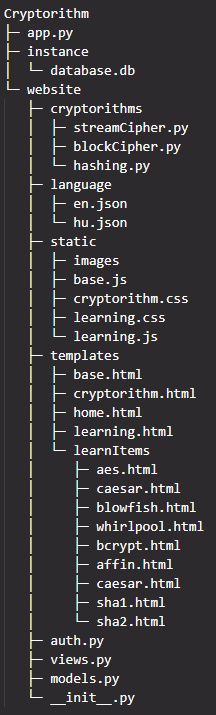
\includegraphics[scale=0.8]{images/fájlStruktúra}
	\caption{Rendszer fájl struktúrája}
\end{figure}

\section {Könyvtárak}

\begin{itemize}
  	\item\textbf{Cryptography:}
A Cryptography egy Python könyvtár, amely kriptográfiai funkciókat és algoritmusokat kínál. Ez a könyvtár ideális választás a projektben, mivel számos kriptográfiai műveletet valósíthatunk meg vele, például hashelést, titkosítást és visszafejtést. A Cryptography megbízható és jól dokumentált eszköz a kriptográfiai műveletek biztonságos végrehajtásához. Jelen esetben ennek a könyvtárnak a segítségével lettek kivitelezve a modernebb rendszerek, például az SHA és az AES.

 	 \item\textbf{Flask:}
A Flask egy könnyű súlyú, de erőteljes webes alkalmazások fejlesztésére szolgáló Python mikrokeretrendszer. A projektben a Flask keretrendszert használom a webes alkalmazás felépítéséhez és a kérések kezeléséhez. A Flask könnyen tanulható és rendkívül rugalmas, ami lehetővé tette, hogy könnyedén kialakítsam a vágyott funkciókat és testreszabhasamk az alkalmazást.

 	 \item\textbf{FlaskSQLAlchemy:}
A FlaskSQLAlchemy egy könnyen használható és hatékony ORM (Object-Relational Mapping) könyvtár, amely lehetővé teszi az adatbázis műveletek kezelését a Flask alkalmazásban. Az SQLAlchemy révén a FlaskSQLAlchemy segít az adatbázis kapcsolatok kezelésében, az adatmodell osztályok definiálásában és az adatbázis műveletek végrehajtásában. A FlaskSQLAlchemy használata átlátható és hatékony adatbázis-interakciókat tesz lehetővé a projektben.

 	 \item\textbf{FlaskLogin:}
A FlaskLogin egy hasznos kiegészítő a Flask keretrendszerhez, amely segít az autentikáció és az azonosítás kezelésében a webes alkalmazásban. A FlaskLogin segítségével egyszerűen implementálhattam a felhasználói regisztrációt, bejelentkezést és kijelentkezést a rendszerben. Ez a könyvtár nagyban megkönnyíti a felhasználói munkamenetek kezelését és a hozzáférési jogosultságok ellenőrzését.

 	 \item\textbf{Json:}
A JSON (JavaScript Object Notation) egy könnyen olvasható és írható adatformátum, amely széles körben használatos az adatok strukturált tárolására és átvitelére. A JSON könyvtárat használva a projektben könnyedén kezelhettem a JSON adatokat, például ennek segítségével valósítottam meg a többnyelvűséget.

 	 \item\textbf{Base64:}
A base64 egy olyan kódolási formátum, amely lehetővé teszi bináris adatok átalakítását olvasható szöveggé. A base64 könyvtárat használva a projektben a bináris adatokat konvertálhatjuk base64 formátumba, ami könnyen kezelhető és továbbítható a webes alkalmazásban. Ennek használata szükséges volt, hogy hatékonyan lehessen alkalmazni a Cryptography könyvtárból használt fügvényeket.

 	 \item\textbf{Glob:}
A glob egy Python könyvtár, amely lehetővé teszi a fájl- és mappaútvonalak kezelését. A glob könyvtár segítségével könnyedén kezelhettem a fájlok vagy mappák neveinek gyűjteményét. Bizonyos fájlok helyzetmeghatározásához használtam, például a .json fájlok eléréséhez.

 	 \item\textbf{Os:}
Az os (operating system) egy Python könyvtár, amely lehetővé teszi az operációs rendszerrel kapcsolatos műveletek végrehajtását. Az os könyvtárat használva a projektben könnyedén manipulálhattam a fájlokat és könyvtárak, például ezek létrehozását, törlését vagy módosítását.

 	 \item\textbf{Math:}
A math egy beépített Python könyvtár, amely matematikai függvényeket és konstansokat kínál. A math könyvtárat használva a projektben matematikai műveleteket végezhetünk, például számításokat végezhetünk, véletlenszámokat generálhatunk vagy trigonometriai műveleteket hajthatunk végre. Jelen esetben a Caesar és Affin rejtjelezéseknek implementálásában használtam.

 	 \item\textbf{Hashlib:}
A hashlib egy Python könyvtár, amely hash-függvényeket kínál. A hashlib segítségével a projektben különböző hashelési műveleteket végezhettem, például az SHA hashelést, amelyek a jelszavak biztonságos tárolásában és a megfelelő műveletek elvégézésére használtam.

 	 \item\textbf{Random:}
A random egy beépített Python könyvtár, amely véletlenszámok generálására szolgál. A random könyvtárat használva a projektben véletlenszerű adatokat generálhatunk, például az egyedi azonosítókat a szükséges rendszerekhez.

\end{itemize}


\section {Felhasználói dokumentáció}
%kezdooldal - login/register
%crypt
%learning
